\begin{frame}{Журнал публикации}

\textbf{Proceedings of the ACM on Programming Languages (PACMPL)}

\vspace{0.5cm}

\begin{itemize}
  \item Международный рецензируемый научный журнал, издаваемый \textbf{ACM}
  \item Ориентирован на исследования в области языков программирования и формальных методов
  \item Публикации сгруппированы по ведущим конференциям:
  \begin{itemize}
    \item POPL (Principles of Programming Languages)
    \item OOPSLA (Object-Oriented Programming, Systems, Languages \& Applications)
    \item ICFP (Functional Programming)
  \end{itemize}
  \item Особенность: статьи проходят строгий peer-review, аналогичный топ-конференциям
  \item Индексируется в основных научных базах (Scopus, Web of Science)
\end{itemize}
\end{frame}

\begin{frame}{Рейтинг журнала}
\begin{center}
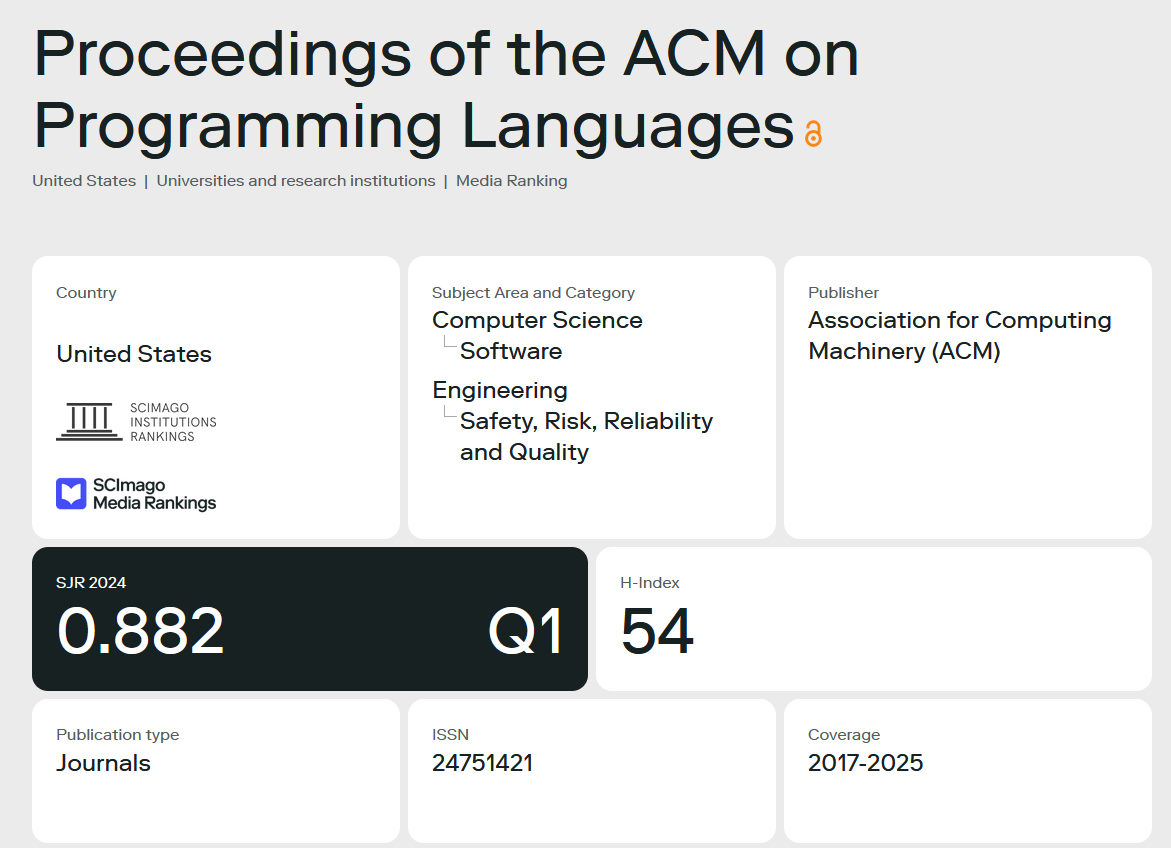
\includegraphics[height=0.9\textheight,keepaspectratio]{figures/journal-score.png}
\end{center}
\end{frame}